\chapter{Introduction}\label{chapter:introduction}
\section{Motivation}\label{section:introduction/motivation}
%This section talks about the context for the problem, highlighting the bigger picture around the problem statement. The general idea about the context.
%not specific about D2worm but about workflow management systems and distributed system, pubsub systems
Business enterprises in current world have complex requirements and expectations in terms of time, speed as well as agility. Increased level of competition in the global market has been one of the key influencing factors for business to be cost effective at runtime, as well as to be open to any future changes. In order to make it possible, enterprises should be agile as much as possible supporting the ability to enhance the business processes along with the underlying information technology.\cite{AMIT-SHETH:1995aa} This insists on the technology infrasturcture capable of incorporating information among various heterogenous systems. \cite{Alonso:2015aa}
\\

Scientific research and experiments are no different than business processes in a way that they require sophisticated infrastructure as well as high processing cabability. Scientific research are no longer limited to single domain or geographical area. Moreover, they need to utilize fresh data as well as services from various interdisciplinary scientific groups with the intension to improve speed, efficiency and accuracy. It clearly suggests that an infrastructure capable of handling large intensive data accross network of scalable systems in a reliable and fast delivery, is required.\cite{Ludascher:2005aa}
\\

The valid requirements discussed in previous segments are fulfilled by workflow management system (\acrshort{WMS}). It is a well-build technology to automate, monitor and controll business processes. It provides the required infrastructure to model the business processes or workflows, generate workflow implementation from the model and monitor the workflow providing required inputs to optimize the business process. It separates the business workflow logic from the core logic and thus provides robust system to define the business process.\cite{AMIT-SHETH:1995aa, Stoilova:2015aa}
\\

Thus, workflow can be considered as the basic element of any \acrshort{WMS}. Depending upon, where wokflow are processesed, a \acrshort{WMS} can be either centralized or distributed. In centralized \acrshort{WMS}, the workflows are modeled as well as executed at central location however in case of distributed or decentralized \acrshort{WMS}, the workflows are distributed across various nodes and executed.\cite{Lee:2000aa} Moreover, the scientific as well as business processes consists of collection of loosely coupled heterogenous computing devices distributed across network spaning to heterogenous domains with different administration control and scalability as well as different performance requirement. \cite{Schneider:2015aa, Alonso:2015aa}
\\

A centralized approach for \acrshort{WMS} cannot be an appropriate choice for such cases but bottleneck and will only increase complexity. \cite{Dogac:2015aa}However, a decentralized workflow management can be the optimum solution. \cite{Alonso:2015aa}
\\

Additionally, depending upon the way workflows are modeled and processed, \acrshort{WMS} can be either activity-centric, document-centric or data-centric. Activity-centric \acrshort{WMS} represents workflow as graph of activities, nodes depicting tasks whereas edges modeling the flow sequence. A slightly improved approach than activity-centric is document-centric approch where workflow are modeled using documents. Both these approaches give high priority to the process-flow rather than the base data model. Also, the static representation of the process-flow makes it hard to change and the complexity of the model increases with the number of tasks. On the other hand, data-centric \acrshort{WMS} uses global data model using application level data and process status information to visualize the workflow. The modeling using business artifacts will provide loose coupling as well as different level of abstraction among agents, which eventually contribute to simplicity and adaptablity.\cite{Jergler:2015aa, Cohn:2015aa}

Taking considerations of all different scenerios and their comparative study as discussed in earlier segments, Distributed Data-centric Workflow On-line Resource Management System (\acrshort{D2WORM}) has been designed and implemented. \acrshort{D2WORM} has a global data model to represent the process state and application data. The overall workflow logic is handled by a coordinated agents or workflow units, each responsible for a part of the complete workflow logic and updating a subset of global data model. Furthermore, the co-ordination among the workflow units is handled by publish-subscribe based network, contributing loose coupling and flexibility.\cite{Jergler:2015aa}
\\


%start
%WorkFlow management system
%why we need it
%distrubuted workflow management system
%datacentric workflow management systems

\section{Problem Statement}\label{section:introduction/problemStatement}
%This section talks about the core problem statement.
%This section defines the problem or the problems this thesis addresses. Basically, this section answers the questions: 
%What is the problem addressed?
%Why is this an important, relevant, and interesting problem? 
%Why is the problem non-trivial, i.e., what are the research challenges that were addressed in this thesis?
%What are the two to three approaches most closely related and how do they differ? Note, this is not the related work analysis that is %presented in a separate chapter.
%This section also defines and discusses the metrics applied to evaluating the approach to  solving the problem defined.


\begin{comment}
\section{Motivation}\label{section:introduction/motivation}
%software architecture and its objectives, relating to responding to the change
Software Architecture definition is an inevitable and crucial step for software development process. By defining an architecture, we define elements, their behavior, their structural composition to construct a system as a whole and various interfaces to characterize communication required between the elements. \cite{microsoft1501} The objective of building an architecture is not only to provide the desired functionalities but also to calibrate the quality of the software across various non-functional attributes such as availability, usability, performance etc. Modifiability is one among the various other quality attributes controlled by an architecture. \cite{Wesley0301}


Software development process as well as development pattern play an equal role to define quality attributes. The quality attributes can be broadly classified as a)Structural and b)Process quality attributes. The structural quality attributes such as testability, modifiability, security etc are affected by the development pattern followed by developers. Adoption of a specific design pattern to solve a problem may be one example of a significant development approach. Similarly, the quality attributes are affected differently, based on the development methodology used. For example, an agile methodology will help to improve maintainability due to its approach of getting fast customer response.\cite{Chappell01}

%change as the most probable expectation and impact of change
Software change is unavoidable for many reasons. The changes are driven by difference between the software’s ability and expectations along time. Additionally, the focus on growing the software require it to undergo changes. Another reason can be to nullify the technical debt occurred along the development stages due to various compromising decisions made.\cite{elsevier0901}
A research carried out by Agile Manifesto, whose result is shown by figure\ref{fig:requirementmismatch} suggests that a surprisingly higher percentage of projects actually fail to meet the requirements of the user.
\begin{figure}[H]
\begin{center}
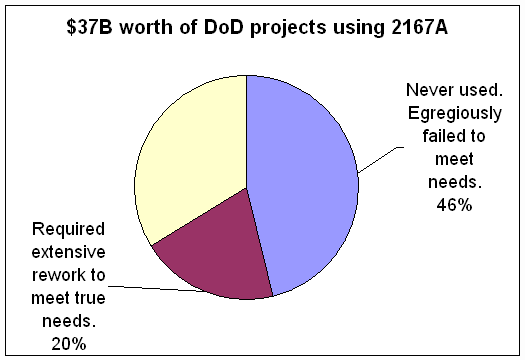
\includegraphics[width=0.8\textwidth]{figures/introduction-motivation}
\caption{Percentage of Projects with Requirement mismatch \cite{Miyachi01}}
\label{fig:requirementmismatch}
\end{center}
\end{figure}
However, responding to change is not free and impose significant impact on software architecture and development methodology. The purpose of architecture and development methodology should be to incorporate those changes and lower the technical debt as swiftly as possible.\cite{Northrop1501} Any variation to software architecture affects coupling and cohesion and thus impacting understandability as well as complexity of the software.\cite{elsevier0901}

The software development methodologies have come a long way undergoing a lot of modifications. Few of them to list would be waterfall model, spiral model, \acrshort{RAD} model and iterative model.\cite{CMS0801} Nevertheless, we have agile modeling, which works around some basic principles. Accepting change requirement at any stage of development and releasing software regularly are among the principles which supports to reduce the the cost of change.\cite{StellmanGreene1401}	

%evolution of the software architecture and development methodology %SOA and microservices
Accordingly, software architecture has changed in number of ways and in number of direction throughout the history of evolution. It has passed through monolithic, layered, distributed object, domain driven development, hexagonal, service oriented architecture etc. \cite{Sommerville0401} Nonetheless, we have microservices architecture with one of the major driving concepts being to improve cohesion and decrease coupling among components. This eventually, apart from accomplishing various other major goals, also upgrades the rate and efficiency of customizability.\cite{Newman1501}

%orchestration micro service is not an exception to that
Microservices are achieved by breaking down a system along business domains following Single Responsibility Principle. As the individual microservices achieved in such a way become the autonomous components, there is a need for a separate kind of component micro service in order to fulfill high-level business goals, which is Orchestration microservice. \cite{Newman1501} Regardless of following agile development methodology and microservice architecture, orchestration has been a painful and cumbersome area, considering the complexities being suffered when one has to make changes at any given point. There are a lot of technological and conceptual procedures around orchestration to make it less painful but at the same time there is no single agreement upon which one to follow.\cite{DanielPernici0601}
\end{comment}
